%%%%%%%%%%%%%%%%%%%%%%%%%%%%%%%%%%%%%%%%%
% Beamer Präsentation
% LaTeX Vorlage
% Version 1.0 (10/11/12)
%
% Diese Vorlage wurde heruntergeladen von:
% http://www.LaTeXTemplates.com
%
% Lizenz:
% CC BY-NC-SA 3.0 (http://creativecommons.org/licenses/by-nc-sa/3.0/)
%
%%%%%%%%%%%%%%%%%%%%%%%%%%%%%%%%%%%%%%%%%

%----------------------------------------------------------------------------------------
%	PAKETE UND THEMEN
%----------------------------------------------------------------------------------------

\documentclass{beamer}

\mode<presentation> {

% Die Beamer-Klasse wird mit einer Reihe von Standard Folienthemen,
% mit unterschiedlichen Farben und Folienlayouts. Nachfolgend eine Liste aller verfügbaren Themen.
% Hier kann das jeweils gewünschte Thema unkommentiert werden.

%\usetheme{default}
% \usetheme{AnnArbor}
% \usetheme{Antibes}
% \usetheme{Bergen}
% \usetheme{Berkeley}
% \usetheme{Berlin}
% \usetheme{Boadilla}
% \usetheme{CambridgeUS}
% \usetheme{Copenhagen}
% \usetheme{Darmstadt}
% \usetheme{Dresden}
% \usetheme{Frankfurt}
% \usetheme{Goettingen}
% \usetheme{Hannover}
% \usetheme{Ilmenau}
% \usetheme{JuanLesPins}
% \usetheme{Luebeck}
 \usetheme{Madrid}
% \usetheme{Malmoe}
% \usetheme{Marburg}
% \usetheme{Montpellier}
% \usetheme{PaloAlto}
% \usetheme{Pittsburgh}
% \usetheme{Rochester}
% \usetheme{Singapore}
% \usetheme{Szeged}
% \usetheme{Warsaw}

% Neben verschiedenen Themen kommt die Beamer-Klasse auch mit diversen Farbvarianten
% für jedes Folienthema daher. Hier kann das jeweils gewünschte Farbthema unkommentiert werden.

% \usecolortheme{albatross}
% \usecolortheme{beaver}
% \usecolortheme{beetle}
% \usecolortheme{crane}
\usecolortheme{dolphin}
% \usecolortheme{dove}
% \usecolortheme{fly}
% \usecolortheme{lily}
% \usecolortheme{orchid}
% \usecolortheme{rose}
% \usecolortheme{seagull}
% \usecolortheme{seahorse}
% \usecolortheme{whale}
% \usecolortheme{wolverine}

%----------------------------------------------------------------------------------------
%	DEFINITION BENUTZERDEFINIERTER FARBEN (RGB)
%----------------------------------------------------------------------------------------
\definecolor{dunkelgrau}{rgb}{0.8,0.8,0.8}
\definecolor{hellgrau}{rgb}{0.95,0.95,0.95}
\definecolor{hellblau}{rgb}{0.8,0.85,1}
\definecolor{dunkelblau}{rgb}{0,0,0.9}

% \setbeamertemplate{footline}				% Zum Entfernen der Fusszeile auf allen Folien kann diese Zeile unkommentiert werden
\setbeamertemplate{footline}[frame number]		% Zum Ersetzen der Fußzeile mit einem einfachen Folienzähler kann diese Zeile auskommentiert werden

\setbeamertemplate{navigation symbols}{}		% Zum Anzeigen der Navigationssymbole am unteren Rand aller Folien kann diese Zeile auskommentiert werden
}

\setbeamertemplate{background canvas} [vertical shading][top=hellblau, bottom=white] 

% \usepackage{pgfpages}				% Zum Erstellen vernünftiger Ausdrucke/Handouts diese Zeile(n) unkommentieren
% \pgfpagesuselayout{resize to}[a4paper,border shrink=5mm,landscape]	% Einseitiger Ausdruck auf A4
% \pgfpagesuselayout{2 on 1}[a4paper,border shrink=5mm]			% Druckt 2 Folien auf 1 Seite A4
% \pgfpagesuselayout{4 on 1}[a4paper,border shrink=5mm,landscape]		% Druckt 4 Folien auf 1 Seite A4
% \pgfpagesuselayout{8 on 1}[a4paper,border shrink=5mm]			% Druckt 8 Folien auf 1 Seite A4
% \pgfpagesuselayout{16 on 1}[a4paper,border shrink=5mm,landscape]		% Druckt 16 Folien auf 1 Seite A4

% \setbeameroption{show notes on second screen=right}	% Zum Anzeigen von Notizen auf dem 2. Schirm.  Mit <location> = left, right, bottom oder top
									% Benötigt das Paket pgfpages!

%\beamerdefaultoverlayspecification{<+->}		% Aufzählungen immer schrittweise zeigen

% \setbeamercovered{transparent}			% Sorgt dafür, daß versteckte Textteile nicht unsichtbar, sondern mit wenig Kontast dargestellt werden

\setbeamerfont{frametitle}{family=\sffamily,series=\bfseries,size={\fontsize{18.00}{20.00}}}	% Setzen der Schriftart und -größe für die Überschriften
\setbeamerfont{footline}{family=\sffamily,series=\bfseries,size={\fontsize{6.00}{7.00}}}		% Setzen der Schriftart und -größe für die Fusszeile

\usepackage[ngerman]{babel}				% für Deutsch
%\usepackage{ngerman}
%\usepackage[english]{babel}				% für Englisch
%\usepackage[latin1]{inputenc}
\usepackage[utf8]{inputenc}
\usepackage{graphicx}					% Erlaubt das Einbinden von Grafiken/Bildern
\usepackage{eurosym}					% Erlaubt das Anzeigen des Eurosymbols
\usepackage{xcolor}					% Erlaubt den Einsatz benutzerdefinierter Farben
								% Weitere Einsatzmöglichkeiten:
								% \textcolor{Farbe}{Text} entspricht Befehlen, wie \textbf{}
								% \pagecolor{Name}, \pagecolor{model}{specification} setzt die Hintergrundfarbe der Seite
								% \colorbox{Name}{Text}, \colorbox{model}{specification}{Text} hinterlegt den Text mit der Farbe
								% \fcolorbox{Name}{Text}, \fcolorbox{model}{specification}{Text} umrandet den Text mit der Farbe
								% vordefinierte Farben: black, white, red, green, blue, cyan, magenta, yellow

\usepackage{colortbl}					% Erlaubt das Verwenden benutzerdefinierter Farben in Tabellen
								% \cellcolor{farbe}, \rowcolor{farbe} oder \columncolor{farbe}

\usepackage{url}						% Erlaubt das Verwenden von URLs ohne umständliche Maskierung
\urlstyle{tt}							% Durch Verwendung von \urlstyle{tt} kann zusätzlich die Schriftart auf Typewriter gestellt werden
\urldef{\fsog}{\url}{http://www.FreieSoftwareOG.org}	% Häufig vorkommende URLs können in einem Makro hinterlegt werden.

\usepackage{booktabs}					% Erlaubt den Einsatz von \toprule, \midrule und \bottomrule innerhalb von Tabellen

% \usepackage{fontspec}					% Erlaubt das Anpassen von Schriftarten. Z.B. auch um eigene Fonts zu verwenden. MUSS MIT XELATEX KOMPILIERT WERDEN!!
% \defaultfontfeatures{Mapping=tex-text}
% \setmainfont{Yanone Kaffeesatz}			% (Haupt-)Schriftart der Präsentation

% Will man ein globales Hintergrundbild verwenden, muss dies in der Preamble definiert werden
% Hier verwende ich das der FSOG
%\usebackgroundtemplate%
%{
%  
\includegraphics[width=\paperwidth,height=\paperheight]{../gemeinsam/Praesentationshintergrund}%
%}

\usepackage{pgf}  
\logo{\pgfputat{\pgfxy(-1.2,-0.2)}{\pgfbox[center,base]{
\includegraphics[width=2.6cm]{../gemeinsam/fsog.png}}}}  

%\logo{
\includegraphics[width=3cm]{../gemeinsam/fsog.png}}




%----------------------------------------------------------------------------------------
% DEFINITION DER TITELFOLIE
%----------------------------------------------------------------------------------------

\title[section77 e.V. - systemd]{systemd} % Der Kurztitel (in eckiger Klammer) erscheint im unteren Bereich aller Folien, der Haupttitel (in geschweifter Klammer) erscheint nur auf der Titelfolie
      
\author{von Justin und Andy}        % Name des Vortragenden
\institute[section77 e.V.]    % Die Institution. Erscheint am unteren Rand aller Folien, zum Platz sparen möglichst eine Abkürzung
{
Community section77 e.V. \\  % Die Institution. Erscheint auf der Titelfolie
\medskip
}
\date{\today}                 % Das Datum des Vortrags (hier: aktuelles Datum)

%----------------------------------------------------------------------------------------
% ANFANG DES DOKUMENTES / DER PRÄSENTATION
%----------------------------------------------------------------------------------------

\begin{document}

\begin{frame}      % Der Zusatz [plain] sorgt dafür, daß keine Seitenzahl/Fusszeile verwendet wird
  \titlepage        % Ausgabe der Titelfolie als erste Folie
\end{frame}

% \begin{frame}         % Inhaltsfolie. Zum Anzeigen können diese Zeilen (von \begin bis \end) unkommentiert werden
% \frametitle{Inhalt der Präsentation}  % Wenn innerhalb der Präsentation \section{} und \subsection{} Befehle verwendet werden,
% \tableofcontents        % werden diese automatisch in diese Inhaltsfolie aufgenommen
% \end{frame}

%------------------------------------------------------------------------------------------
% AB HIER BEGINNT DIE EIGENTLICHE PRÄSENTATION
%------------------------------------------------------------------------------------------

\begin{frame}
\frametitle{was ist systemd?}
ein Daemon, der als Init-Prozess - als erster Prozess - zum Starten, Überwachen
und Beenden weiterer Prozesse dient.

In den Standard-Distros inzwischen enthalten und dort zum Default geworden:

\begin{itemize}
  \item SLES (seit 12)
  \item Debian (seit 8)
  \item Ubuntu (seit 15.04)
  \item Fedora (seit 15)
  \item OpenSuse (seit 12.1)
  \item RHEL (seit 7)
  \item Arch (seit Okt. 2012)
\end{itemize}

\end{frame}

\begin{frame}
  \frametitle{Vorteile}
  \begin{itemize}
    \item höhere Geschwindigkeit beim Start des Systems durch parallel gestartete
          Prozesse. Dies macht besonders bei Mehrkernprozessoren Sinn
    \item systemd kümmert sich um eine Strategie wie die Prozesse nacheinander
          gestartet werden können. Der Anwender gibt einfach nur an welche anderen Prozesse benötigt werden
    \item vereinfachte Schnittstelle zur Steuerung der Dienste und Betrachtung der Logfiles
  \end{itemize}
\end{frame}

\begin{frame}
  \frametitle{Nachteile}
  \begin{itemize}
    \item bricht das Basiskonzept "ein Programm soll ein Problem lösen, dieses aber möglichst gut". 
    \item speichert Logdateien im Binärformat, nicht als Text
    \item systemd wurde schon mehrfach nachgesagt, es spalte die Community (Stichwort Devuan). Teilweise richtet
  sich dies direkt gegen die zwei Haupentwickler. Auch Linus Torvalds hat sich schon zu Wort gemeldet (0day patch)
  \end{itemize}

\end{frame}

\begin{frame}[fragile]

\frametitle{Vergleich: Kommando bei init/systemd}

  Start eines Dienstes
  \begin{itemize}
    \item init:
    \begin{verbatim}
    $ /etc/init.d/apache2 start
    \end{verbatim}

    \item systemd:
    \begin{verbatim}
    $ systemctl start apache2
    \end{verbatim}
  \end{itemize}

\end{frame}

\begin{frame}[fragile]
\frametitle{Vergleich: Kommando bei init/systemd}

  Aktivieren eines Dienstes (automatischer Start beim Boot):
  \begin{itemize}

    \item RedHat-Style:
    \begin{verbatim}
    $ chkconfig 235 httpd
    \end{verbatim}

    \item SysVinit-Style:
    \begin{verbatim}
    $ ln -s /etc/init.d/apache2 /etc/rc2.d
    # (und das Ganze nochmal für die runlevel 3 und 5)
    \end{verbatim}

    \item systemd:
    \begin{verbatim}
    $ systemctl enable apache2
    \end{verbatim}

  \end{itemize}

\end{frame}


\begin{frame}[fragile]
\frametitle{Status/Logging}

  \begin{itemize}

    \item Ohne systemd:
    \begin{verbatim}
    $ less /var/log/...
    \end{verbatim}
    oder mit grep in den logfiles suchen

    \item Mit systemd:
    \begin{verbatim}
    $ systemctl status apache2
    $ journalctl -u apache2
    $ journalctl -p err..alert
    \end{verbatim}

  \end{itemize}

\end{frame}

\begin{frame}
  \note[item]{Wear-Leveling = Daten werden gleichmäßig verteilt}
  \note[item]{Sicher ist es also nur, wenn der gesamte Flash-Speicher überschrieben wird}
  \frametitle{Stolperstein:\\Flash-Speicher (SSDs und USB-Sticks)}
  \begin{itemize}
    \item Verhalten ist stark Fabrikats- bzw. Herstellerabhängig
    \item Grundsätzlich ist es nicht möglich, gezielt Blöcke auf dem Speicher zu überschreiben
    \item Schreibzyklen sind (je nach Bauart) begrenzt
    \item Deshalb wird Wear-Leveling vom integrierten Controller verwendet
    \item Moderne Flash-Speicher verwenden eine interne Garbage Collection des Controllers
    \item oder den TRIM-Befehl des Betriebssystems
  \end{itemize}
  \pause
  \begin{alertblock}{Deshalb}
    {\bf Verschlüsseln} (Einzelne Dateien oder ganze Partition).
  \end{alertblock}
\end{frame}

\begin{frame}
  \note[item]{Defekte Sektoren werden solange nicht bemerkt, wie noch Erstzsektoren bereit stehen.}
  \frametitle{Stolperstein:\\Defekte Sektoren}
  \begin{itemize}
    \item Controller verwaltet diese gegenüber dem Betriebssystem transparent
    \item Daten in defekten Sektoren bleiben erhalten
    \item Kontrolle vorhandener defekter Sektoren ist möglich
    \begin{itemize}
      \item mit \textit{smartmontools}
      \item z.B. \textit{smartctl -a sda}
      \item z.B. \textit{smartctl -a sda  grep Reallocated\_Sector\_Ct}
    \end{itemize}
  \end{itemize}
\end{frame}

\begin{frame}
  \note[item]{Nochmal Hinweis auf Verschlüsselung}
  \frametitle{Stolperstein:\\Journaling}
  \begin{itemize}
    \item ext3/4 sowie reiserfs erstellen ein Meta-Journal
    \item Manche Dateisysteme und Journal-Modi speichern sogar ganze Dateien im Journal, welche dann auch aus dem Journal wieder rekonstruiert werden können, obwohl sie auf der Festplatte vollständig gelöscht und sogar mit wipe überschrieben wurden...
  \end{itemize}
\end{frame}

\begin{frame}
  \note[item]{MBR muss im Schadensfall (Trojaner, etc.) neu angelegt werden. Dann aber auch keine Rekonstruktion mehr möglich!}
  \frametitle{Stolperstein:\\MBR (Master Boot Record)}
  \begin{itemize}
    \item Das Löschen einzelner Dateien oder Verzeichnisse hat keinen Einfluss auf diesen Bereich
    \item Schadprogramme setzen sich hier fest
    \item Löschen von Partitionen bzw. Formatieren der Festplatte nützt nichts
  \end{itemize}
\end{frame}

\begin{frame}
  \frametitle{Löschmethoden}
  \begin{itemize}
    \item Gutmann-Methode (1996)
    \item Russian GOST P50739-95
    \item Bruce Schneier's Algorithm
  \end{itemize}
\end{frame}

\begin{frame}
  \frametitle{Die Mär vom 35-fachen Überschreiben}
  Ist es wirklich notwendig, einen Datenträger 35-fach zu überschrieben, um sicher zu sein, daß nichts mehr rekonstruierbar ist?
  \pause
  \begin{alertblock}{Craig Wright behauptet}
    {\bf NEIN!} (Studie von 2009).
  \end{alertblock}
  \pause
  Bereits das einmalige Überschreiben lässt keine Chance für Forensiker
\end{frame}

\begin{frame}
  \note[item]{shred: Arbeitet nach Gutmann-Methode, kann keine Ordner löschen.}
  \note[item]{Secure Remove: Steht für Debian/Ubuntu im Paket secure-delete bereit.}
  \frametitle{Werkzeuge für sicheres Löschen\\(einzelne Dateien)}
  \begin{itemize}
    \item shred
      \begin{itemize}
        \item shred -vun \textit{Durchgänge} \textit{Datei1  Datei2}
        \item find \textit{Verzeichnis} -type f -print0 \textbar ~xargs -0 shred -vun \textit{Durchg.}
      \end{itemize}
    \item wipe
      \begin{itemize}
        \item wipe \textit{datei.jpg}
        \item wipe -r \textit{Ordner/}
      \end{itemize}
    \item Secure Remove
  \end{itemize}
\end{frame}

\begin{frame}
  \frametitle{Werkzeuge für sicheres Löschen\\(ganze Datenträger)}
  \begin{itemize}
    \item dd
      \begin{itemize}
        \item dd \path{if=/dev/zero} \path{of=/dev/sda}
        \item dd \path{if=/dev/urandom} \path{of=/dev/sda}
      \end{itemize}
    \item shred
      \begin{itemize}
        \item shred -vn \textit{Durchgänge} \textit{Gerät}
      \end{itemize}
    \item wipe
      \begin{itemize}
        \item wipe -k \path{/dev/sda7}
      \end{itemize}
    \item Plattenputzer
    \item DBAN
  \end{itemize}
\end{frame}

\begin{frame}
  \frametitle{Werkzeuge für sicheres Löschen\\(ganze Datenträger)}
  %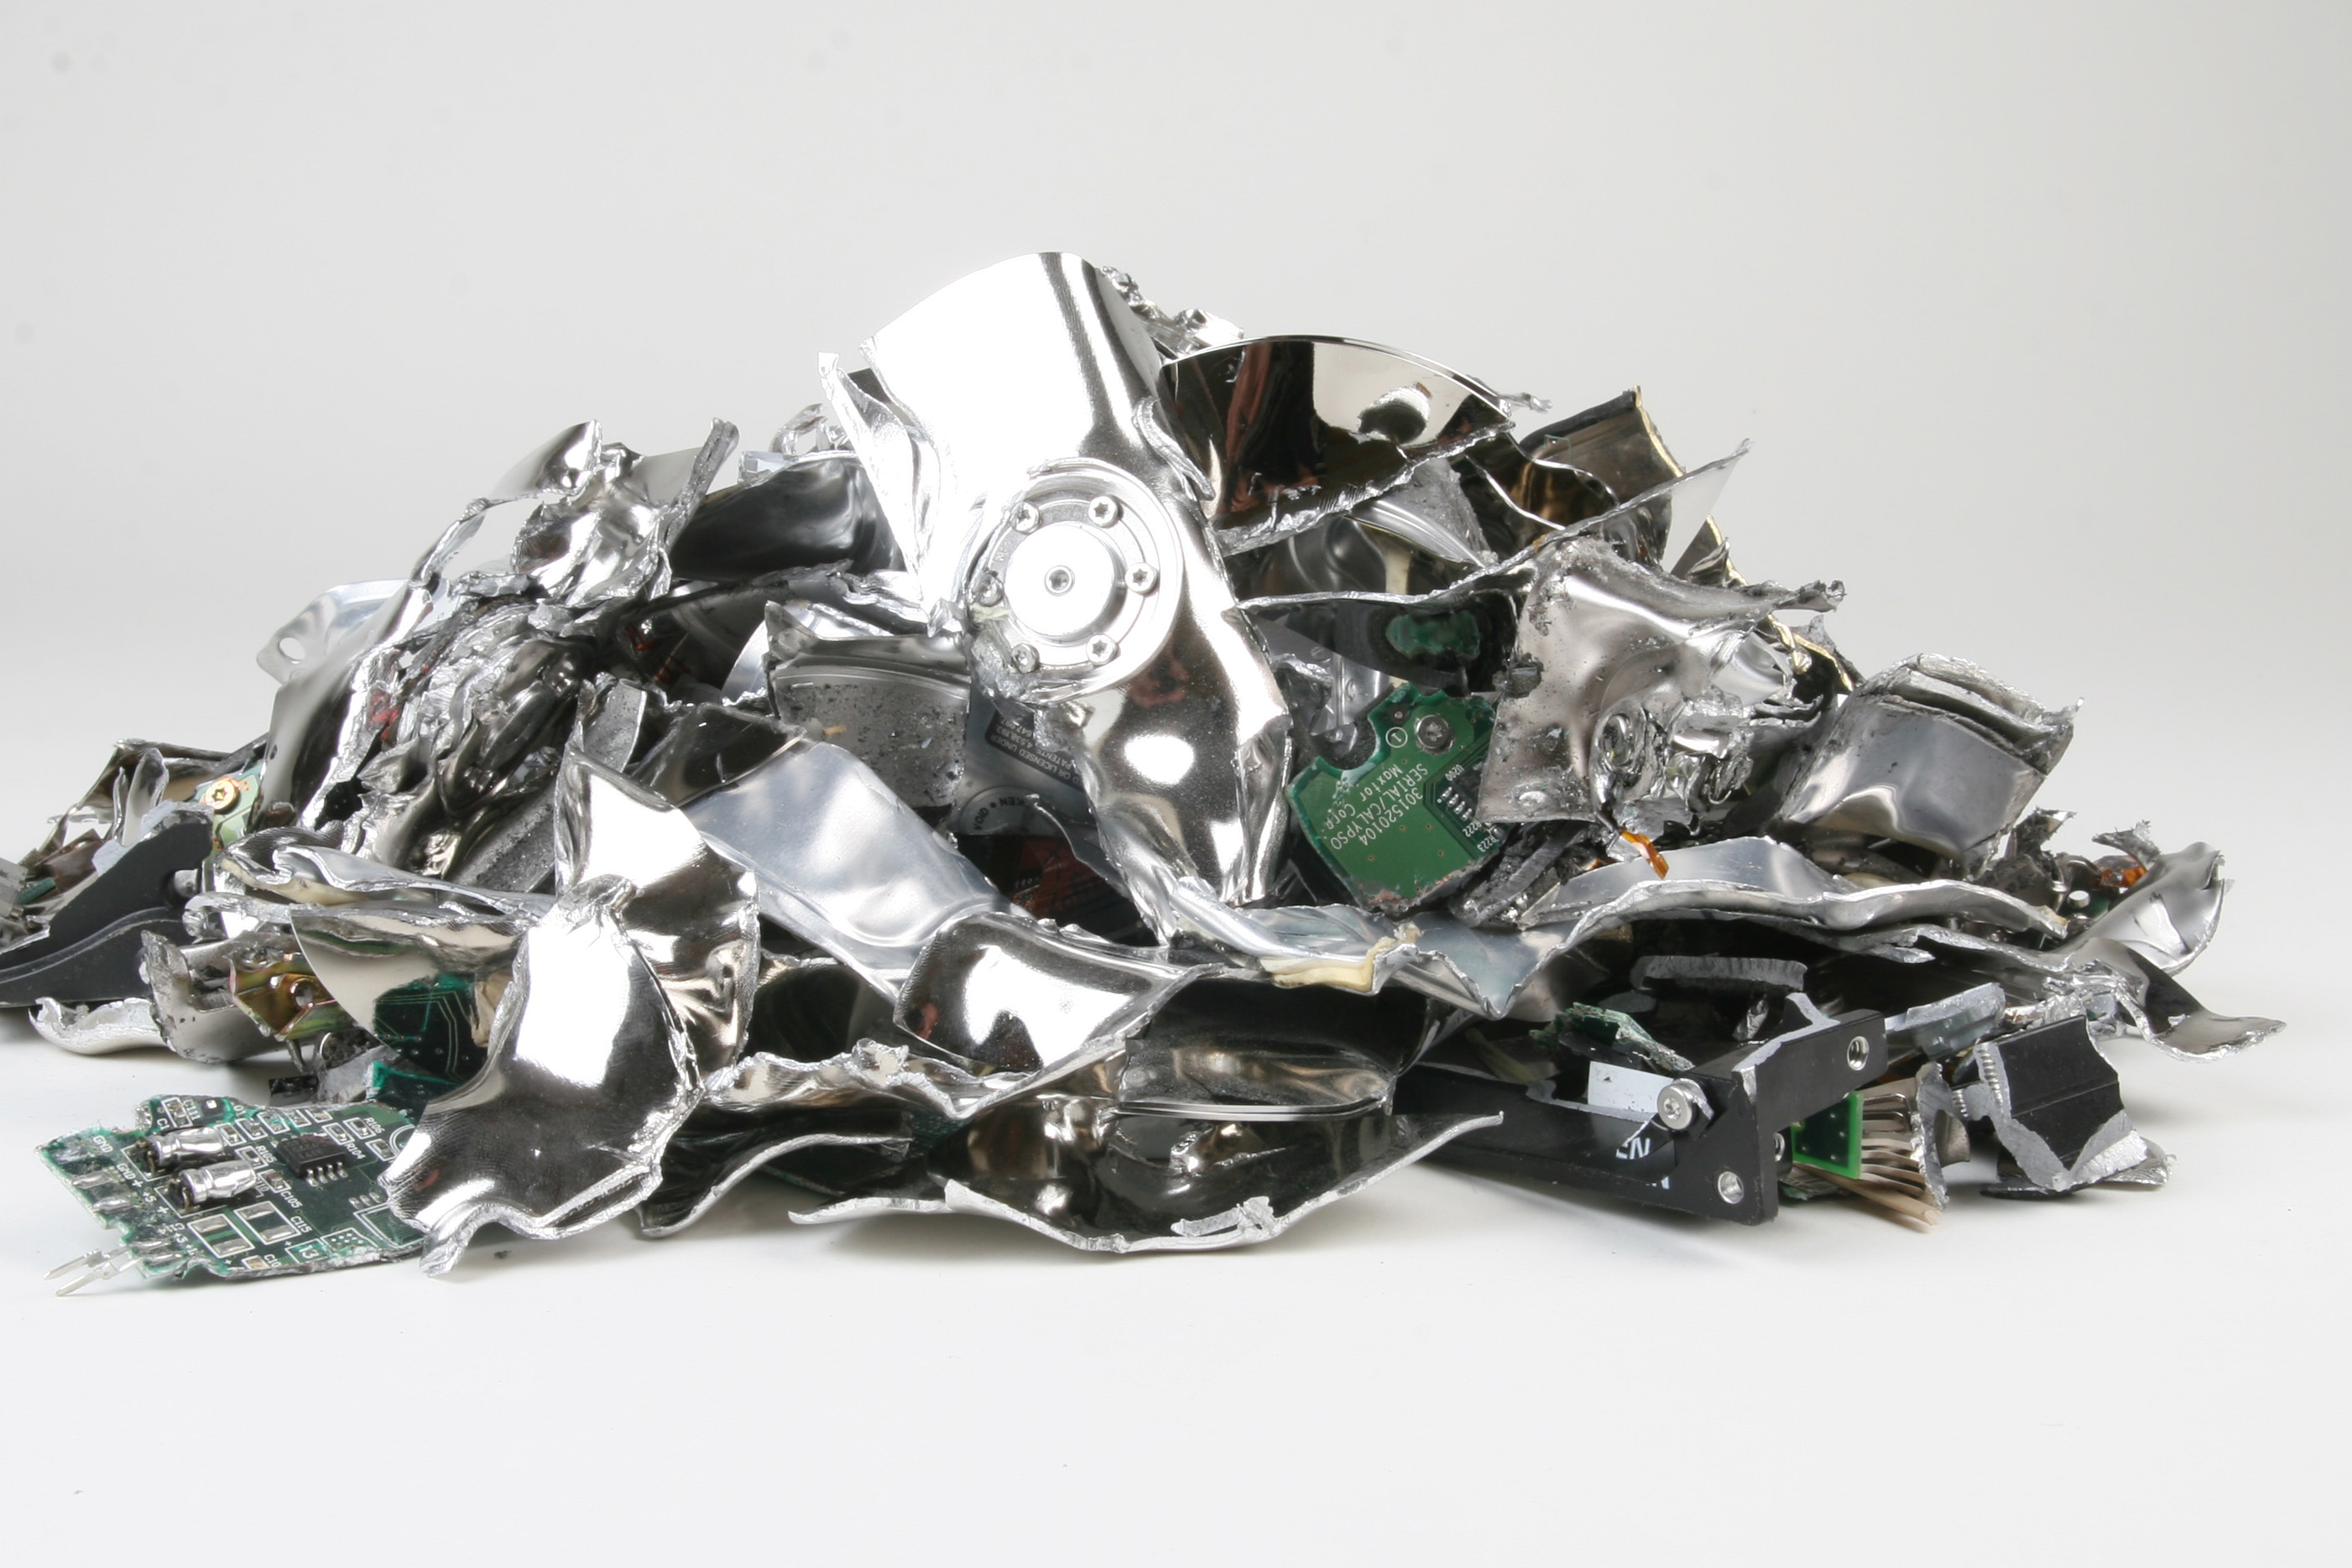
\includegraphics[width=0.9\linewidth]{Bilder/HDDFragmente}
\end{frame}

\begin{frame}[fragile]   % Die "fragile"-Option muss verwendet werden, wenn auf der Folie verbatim verwendet wird
\frametitle{Links zur Präsentation}
  \begin{verbatim}
    http://www.linux-magazine.com/Issues/2017/200/Tutorials-Systemd
    https://wiki.debian.org/systemd/Services
  \end{verbatim}
\end{frame}

\begin{frame}
\frametitle{Weitere Informationen bekommen Sie hier:}
  \begin{center}
  \Large{
    \fsog \\      % Makro für das Einfügen der URL (oben definiert)
    und \\
    Kontakt@FreieSoftwareOG.org \\~\\

    oder kommen Sie doch einfach zu unserem regelmäßigen Treffen, \\
    jeden 1. Mittwoch im Monat ab 20:00 Uhr. \\
    (Treffpunkt und Thema laut Webseite)
    }
  \end{center}
  \begin{figure}[ht]
    \centering
    
\includegraphics[width=0.2\textwidth]{../gemeinsam/CC-BY-SA.png}
  \end{figure}  
\end{frame}
\end{document}
